\documentclass{article}
\usepackage[utf8]{inputenc}
\usepackage{amsmath}
\usepackage{hyperref}
\usepackage{graphics}


\begin{document}

\section{Free Energy Calculation Using Q}

Free energy perturbation (FEP) calculations with Q involves running a set of consecutive input files which have the mapping parameter $\lambda$ ranging in a way (usually [1, 0] to [0, 1] between two states). Qfep is a program which reads the energy files generated by Qdyn and calculates the total change in free energy for the complete perturbation from state A ($\varepsilon_1$) to state B ($\varepsilon_2$). Zwanzig’s formula as shown below calculates the difference in free energy between the two states:

\begin{equation}
    \Delta G = \sum \Delta g = \sum -R \cdot T \cdot \ln \left\langle e^{-\left(\frac{\Delta V_{\text{eff}}}{R \cdot T}\right)} \right\rangle_{A}
\end{equation}

Here, \(\Delta V_{\text{eff}}\) is defined as the difference in \( V_{\text{eff}} \) between two adjacent perturbation steps. 

Qfep also calculates free energy functions, or potentials of mean force, using the perturbation formula. The reaction coordinate \(X\) is defined as the energy gap between the states \(X = \Delta V = \varepsilon_1 - \varepsilon_2\) and is divided into intervals \(X_m\) (bins). The first term in the equation represents the free energy difference between the initial state \(\varepsilon_1\) and the mapping potential \(V_i\):

\begin{equation}
    \Delta G(X_m) = \Delta G (\lambda_i) - R \cdot T \cdot \ln \left\langle e^{-\left(\frac{E_g(X_m) - V_i(X_m)}{R \cdot T}\right)} \right\rangle_{i}
\end{equation}

The second term represents the free energy difference between the mapping potential \(V_i\) and the ground state potential \(E_g\). The average in this term is taken over those configurations where \(X\) belongs to \(X_m\).

\begin{equation}
    \Delta G(\lambda_i) = - R \cdot T \cdot \ln \left( \sum_{n=0}^{i-1} \left\langle e^{-\left(\frac{V_{n+1} - V_n}{R \cdot T}\right)} \right\rangle_{n} \right)
\end{equation}

\(E_g\) is the solution to the secular determinant. The system is then represented by an \(n \times n\) EVB Hamiltonian.

\[ 
  \left[\begin{array}{cc}
    H_{11} & H_{12} \\
    H_{21} & H_{22} \\
  \end{array}\right]
\]

Here, \(H_{11}\) and \(H_{22}\) are the energies of the two valence states which are calculated using classical force fields. 
For a two-state representation, the solution becomes:

\begin{equation}
    E_g = \frac{1}{2} \cdot \left( \epsilon_1 + \epsilon_2 \right) - \frac{1}{2} \sqrt{ \left( \epsilon_1 - \epsilon_2 \right)^2 + 4 \cdot H_{12}^2 }
\end{equation}

where \(H_{ij}\) or \(H_{12}\) is the off-diagonal matrix element representing the quantum mechanical coupling of the states. \(H_{ij} \neq 0\) results in the mixing of states \(i\) and \(j\). In Qfep, the off-diagonal element \(H_{ij}\) is a function of the form:

\begin{equation}
    H_{ij} = A_{ij} \cdot e^{-(\mu (r_{ij} - r_0) + \eta (r_{ij} - r_0)^2)}
\end{equation}

The EVB method allows calibration of simulated reference reactions to experimental data obtained from gas-phase or solution experiments. The two EVB parameters \(H_{ij}\) (mostly \(A_{ij}\)) and \(\Delta \alpha\) are adjusted in a way until the calculated profile and the experimental data coincide. The \(\Delta \alpha\) parameter determines the \(\Delta G^\circ\) level, and \(H_{ij}\) regulates the degree of mixing of the states at the transition state, i.e., the \(\Delta G^\ddagger\) level.


\section{Computational Methodology}

The first step in preparing a simulation that has missing force field parameters along with standard parameters and library files. In this case it is Selenium (U). After equilibration, continuing with the FEP simulations which constitute the core part of the EVB methodology. The FEP protocol involves a gradual change of the (mapping) potential energy by the coupling parameter lambda. This change of potential will drive the system from the region of configurational space corresponding to the reactant state (RS) to that corresponding to product state (PS). The MD simulation required for a free energy calculation often proceeds in multiple stages. The initial stage is running at a very low temperature with strong coupling to the temperature bath (energy minimisation) to relax strain in the initial structure. Following stepwise heating of the simulated system and equilibration at the target temperature. For perturbation simulations, this phase is composed of a series of simulations using intermediate potentials defined by different sets of weight coefficients for the FEP states.

\subsection{Computational Model Preparation}

The initial structure used to make the EVB model was for mouse cysteine wild type (PDB ID - 7FC2) and for human selenocysteine wild type it was generated with alphafold. For creating the selenium parameters (selenol, selenolate ion and selenenic acid) FFLD in maestro [] was used. We used the charges provided by Maestro [], the hydrogen and solvent was added using Q program \cite{Marelius1999}. The TIP3P water parameters were used in combination with the other protein parameters not present in the standard OPLS library in Q mentioned above.

\subsection{EVB simulations}

Spherical boundary conditions \cite{King1989} were applied to the system using Q program \cite{Marelius1999} using 50 \text{\AA} diameter water covering the protein.

\begin{figure}
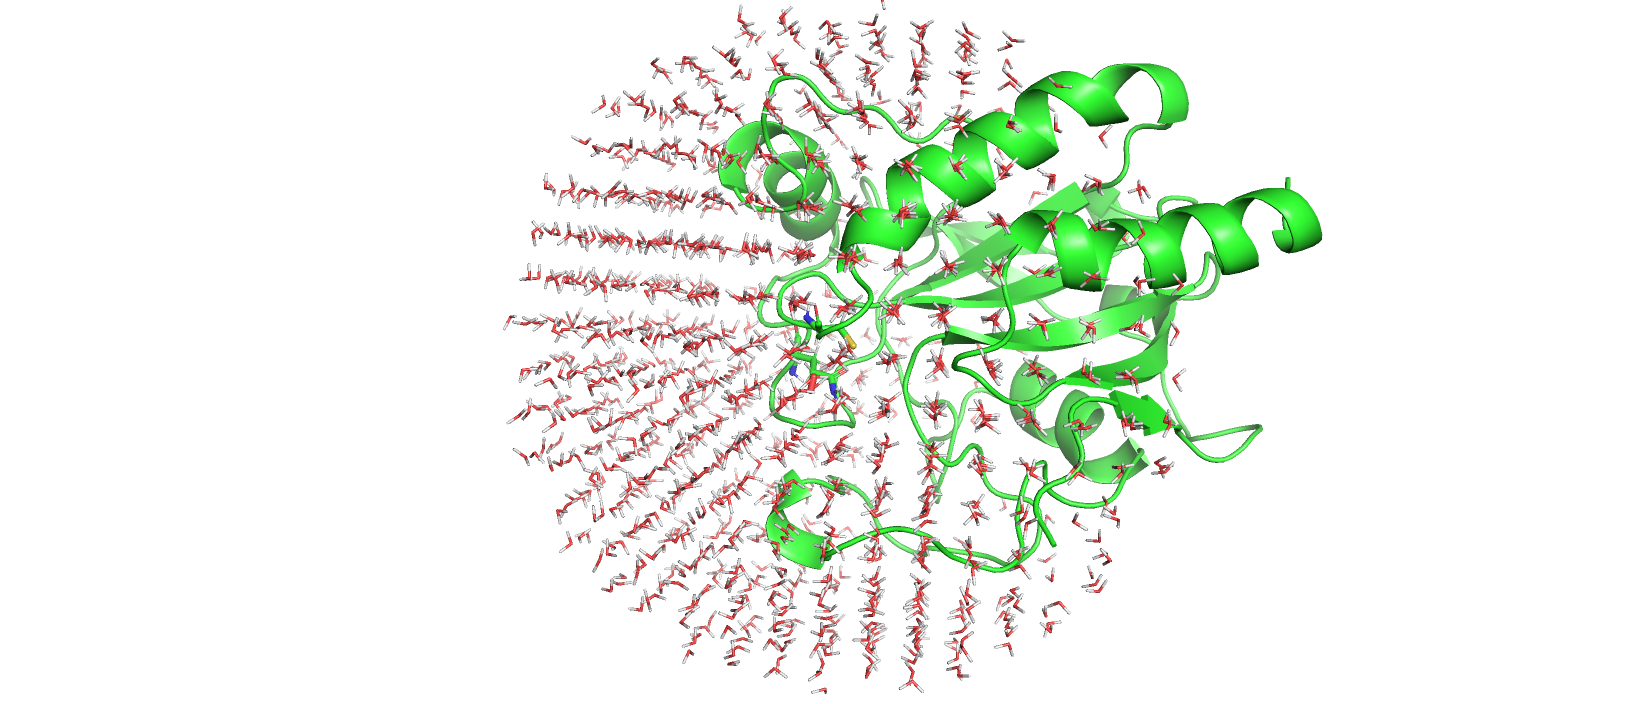
\includegraphics{../figures/solvent_sphere.png} 
\caption{Sphere of Water Molecules around the protein}
\label{fig:figure1}
\end{figure}

After equilibration of the system, two separate MD/EVB free energy perturbation (FEP) calculations were done for the step 1 (until formation of selenolate ion) and the step 2 (to the formation of selenenic acid), which is the product of the reaction. The FEP protocol involves a gradual change of the (mapping) potential energy by the coupling parameter. For each of the FEP calculations, 51 decreate windows were considered, each window of 10 ps at 2 fs time step, that gave a total of 1.02 ns of sampling of each free energy profile . These calculations were replicated 100 times starting from the minimized structure. The EVB gas phase shift $\alpha$  and the off diagonal Hij were determined iteratively. in order to have an average reaction free energies and the barrier heights of all the four systems in study. The four barriers we got were essentially determined according to the QM/MM calculations that have been previously done.(TS1 - 16.4 kcal/mol and Product - 18.8 kcal/mol)


\medskip

%Sets the bibliography style to UNSRT and imports the 
%bibliography file "references.bib".
\bibliographystyle{unsrt}
\bibliography{references}




\end{document}
